
\section{Background}\label{sec:background}

In recent years, the field of computer vision has been growing in complexity and the number of applications has been increasing, main applications are: image classification, object detection, face recognition, image segmentation, \gls{slam} and visual odometry which is a task in which the robot is able to understand where it is and how it is oriented.

The development of computer vision has been a long process, the growth is favoured by the development of new hardware components and new challenges, about the latters, we have
CIFAR-10 (Doon et al.~\cite{cifar10_paper}), Fashion-MNIST(Xiao et al.~\cite{fashion_mnist_paper}), MS-Coco (Lin et al.~\cite{ms_coco_paper}) and ImageNet (Deng et al.~\cite{imagenet_paper}).
These datasets are often used as benchmark for novel models.

For the architectures, starting from AlexNet (Krizhevsky et al.~\cite{alex_net_paper}), then VGG (Simonyan et al.~\cite{vgg_paper}), Inception-V1 (Szegedy et al.~\cite{inception_v1_paper}), Inception-V2(Szegedy et al.~\cite{inception_v2_paper}), ResNet (He et al.~\cite{resnet_paper}), etc., the complexity of the models has increased enormously.
Each of these models introduced some innovations and improved the performance on the benchmarks, for example:
\begin{itemize}
    \item AlexNet introduced the concept of the \emph{convolutional neural network} (CNN) and use of the separation of the models into two different GPUs.
    \item VGG introduced the concept of stage, which repeated more times, composes the model.
    \item Inception-V1, Inception-V2 and V3 which are based on the concept of \emph{inception module} which was composed by different paths that the input has to go through to reach the output.
    \begin{figure}[H]
        \centering
        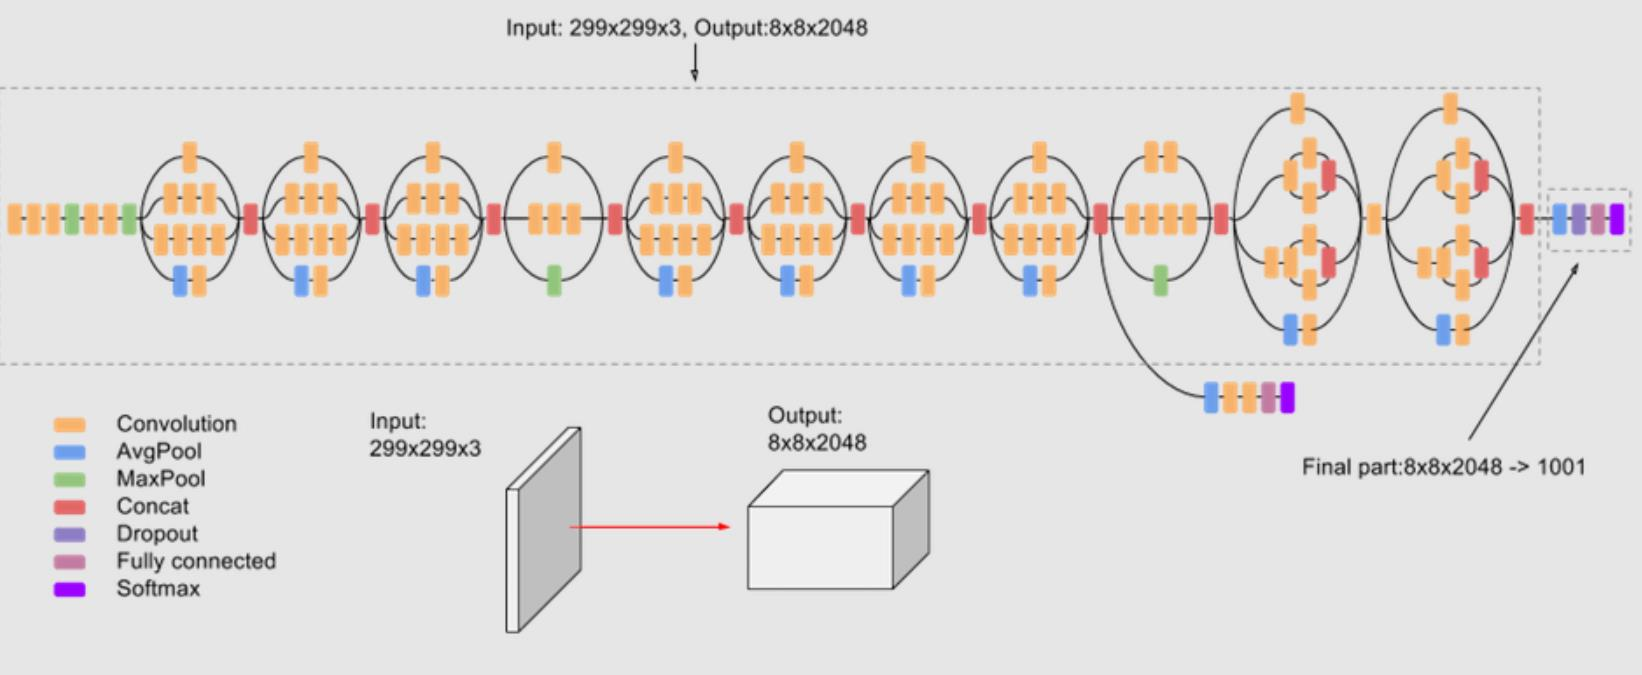
\includegraphics[width=\textwidth]{images/1_inception_v3}
        \caption{Inception V3 Structure}\label{fig:inception-v3}
    \end{figure}
    \item ResNet is a model that is based on the concept of \emph{residual network} which is composed by several blocks of the same type with the skip connections:
    \begin{figure}[H]
        \centering
        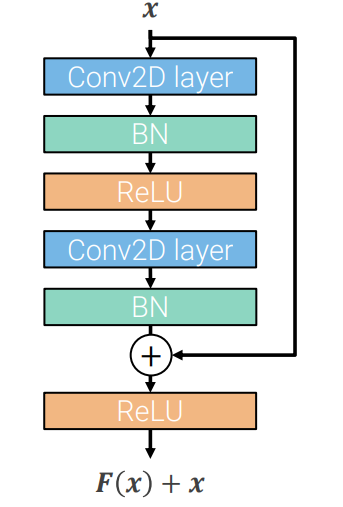
\includegraphics[width=0.4\textwidth]{images/1_1_skip_connection}
        \caption{Skip connection}\label{fig:skip-connection}
    \end{figure}
    Basically, the input of the block is added to the output before feeding it to the next block, in this way, we can avoid the \gls{vanishing gradient problem} making easier the training process.
\end{itemize}
After this, the computer-visionists lend the Transformer architecture (Vaswani et al.~\cite{transformer_paper} from \gls{nlp}, bringing up ViT (Dosovitskiy et al.~\cite{vit_paper}) which is based on the \gls{mha} mechanism.
A multi-head attention is a module for attention mechanisms which runs through an attention mechanism several times in parallel.
In this way, the model can attend to the different parts of the input, forming, in this way, the cross-attention over different parts of the input.
